%%%%%%%%%%%%%%%%%%%%%%%%%%%%%%%%%%%%%%%%%
% University Assignment Title Page 
% LaTeX Template
% Version 1.0 (27/12/12)
%
% This template has been downloaded from:
% http://www.LaTeXTemplates.com
%
% Original author:
% WikiBooks (http://en.wikibooks.org/wiki/LaTeX/Title_Creation)
%
% License:
% CC BY-NC-SA 3.0 (http://creativecommons.org/licenses/by-nc-sa/3.0/)
% 
% Instructions for using this template:
% This title page is capable of being compiled as is. This is not useful for 
% including it in another document. To do this, you have two options: 
%
% 1) Copy/paste everything between \begin{document} and \end{document} 
% starting at \begin{titlepage} and paste this into another LaTeX file where you 
% want your title page.
% OR
% 2) Remove everything outside the \begin{titlepage} and \end{titlepage} and 
% move this file to the same directory as the LaTeX file you wish to add it to. 
% Then add \input{./title_page_1.tex} to your LaTeX file where you want your
% title page.
%
%%%%%%%%%%%%%%%%%%%%%%%%%%%%%%%%%%%%%%%%%
%\title{Title page with logo}
%----------------------------------------------------------------------------------------
%	PACKAGES AND OTHER DOCUMENT CONFIGURATIONS
%----------------------------------------------------------------------------------------

\documentclass[11pt]{article}
\usepackage[english]{babel}
\usepackage[utf8x]{inputenc}
\usepackage{amsmath, graphicx}
\usepackage[colorinlistoftodos]{todonotes}

\begin{document}

\begin{titlepage}

\newcommand{\HRule}{\rule{\linewidth}{0.5mm}} % Defines a new command for the horizontal lines, change thickness here

\center % Center everything on the page
 
%----------------------------------------------------------------------------------------
%	HEADING SECTIONS
%----------------------------------------------------------------------------------------

\textsc{\LARGE Universidad de Sonora }\\[0.3cm] % Name of your university/college
\textsc{\Large Departamento de Ciencias Naturales y Exactas  }\\[0.3cm]
\textsc{\Large Licenciatura en Física }\\[0.3cm]
\textsc{\Large Física computacional I}\\[0.5cm] % Major heading such as course name
 % Minor heading such as course title

%----------------------------------------------------------------------------------------
%	TITLE SECTION
%----------------------------------------------------------------------------------------

\HRule \\[0.4cm]
{ \huge \bfseries Actividad 1\\  Atmósfera de la Tierra}\\[0.03cm] % Title of your document
\HRule \\[1.5cm]

 
%----------------------------------------------------------------------------------------
%	AUTHOR SECTION
%----------------------------------------------------------------------------------------

\begin{minipage}{0.4\textwidth}
\begin{flushleft} \large
\emph{Alumno:}\\
Gómez García \\Manuel Ignacio\\ %Grupo 1 % Your name
\end{flushleft}
\end{minipage}
~
\begin{minipage}{0.4\textwidth}
\begin{flushright} \large
\emph{Profesor:} \\
Lizarraga Celaya\\Carlos\\%Dept. of CSE % Supervisor's Name
\end{flushright}
\end{minipage}\\[1cm]

% If you don't want a supervisor, uncomment the two lines below and remove the section above
%\Large \emph{Author:}\\
%John \textsc{Smith}\\[3cm] % Your name

%----------------------------------------------------------------------------------------
%	DATE SECTION
%----------------------------------------------------------------------------------------

{\large \date[10 de febrero, 2018 \\Hermosillo, Sonora}\\[1cm] % Date, change the \today to a set date if you want to be precise

%----------------------------------------------------------------------------------------
%	LOGO SECTION
%----------------------------------------------------------------------------------------


\includegraphics[height=7cm]{Logo}\\[1cm] % Include a department/university logo - this will require the graphicx package
 
%----------------------------------------------------------------------------------------

\vfill % Fill the rest of the page with whitespace

\end{titlepage}



\noindent La atmósfera de la Tierra está compuesta principalmente
de gases, gracias a la gravedad del planeta. Es debido a la ella
que existe la vida pues genera presión que da lugar al agua, nos
protege de la radiación emitada por el Sol, disminuyendo así la
cantidad y calentando la Tierra lo necesario.
\\[3mm] El volumen de la atmósfera es un 78.09\% nitrogeno, 20.95\%
oxígeno, 0.93\% argón, 0.04\% dióxido de carbono, y el resto
corresponde a otro tipo de gases.
\\[3mm] La atmósfera cuenta con una masa aproximadamente de
$5.15$x$10^{18}$ kg, de los cuales $\frac{3}{4}$ se encuentran
entre los primeros 11 km de la superficie. A lo largo de ella,
conforme aumenta la altitud, podemos distinguir distintas capas
y que son clasificadas en base a características como su
temperatura y composición. 

\section{Composición}
Los tres mayores constituyentes de la atmósfera son nitrógeno,
oxígeno y argón, mientras quue el vapor de agua apenas representa
el 0.25\%; su concentración varía alrededor de 10 ppm por volumen
en las zonas más heladas hasta 5\% por volumen en las más calientes.
Los gases restantes son rastros del efecto invernadero, siendo estos dióxido de carbono, metano, óxido nitroso, y ozono, así como otro
tanto más de restos químicos provenientes de la contaminación de
gases de origen natural, aerosoles, o bien, por las fábricas.

\section{Estructura de la atmósfera}

En general, la presión y densidad disminuye conforme aumenta la
altitud, sin embargo con la temperatura es algo más complicado
que eso debido a que se mantiene relativamente constante, por lo
cual es necesario medir estos cambios con ciertos dispositivos,
en base a ello se ha dividido la atmósfera en cinco distintas capas.
\\[3mm] La figura 1 ilustra el cómo se han dividen las capas
atmosféricas.

\begin{figure}
\centering
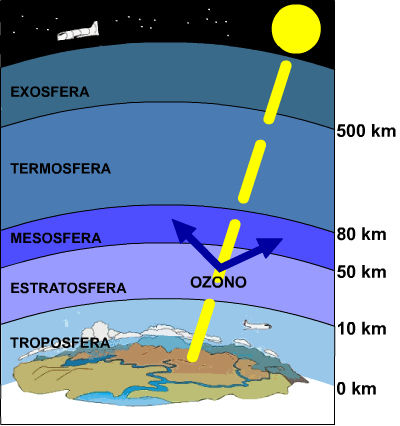
\includegraphics[width=6cm]{CapasAtmosfera}
\caption{\label{capa}Capas de la atmósfera.}
\end{figure}

\subsection{Troposfera}   
La troposfera es la capa de la atmósfera donde habitamos los seres
vivos y abarca cerca de los primeros 12 km de altitud, aunque está             altitud varía según la ubicación (9 km en los polos y 17 km en el               ecuador).
\\[3mm] Aunque ocurren ciertas variaciones, la temperatura desciende                 conforme se asciende a través de la atmósfera ya que existe una transferencia de energía con la superficie del planeta. Contenida
en esta capa encontramos el 80\% de la masa atmosférica y dentro
de los primeros 5.6 km, el 50\% de la masa total, conviertiendo a
ésta en la capa más densa de todas.
\\[3mm] Aquí es donde vuelan las aeronaves propulsadas por hélices.
    
\subsection{Estratosfera}
Esta capa comienza en la tropopausa y termina alrededor de los 50 o
55 km de altitud.
\\ La presión atmosférica en el borde superior de la capa es
$\frac{1}{1000}$ de la presión a nivel del mar. Aquí es donde
encotraremos la capa de ozono, es donde se encuentra una alta
concentración de este gas, es por ello que en esta capa incremente
la temperatura conforme la altitud pues los rayos UV son retenidos
por el gas provocando que la temperatura asciende desde -60 ºC
hasta 0 ºC en la parte superior.
\\[3mm] Esta es el punto más alto a donde pueden llegar las
aeronaves impulsadas por jet.

\subsection{Mesosfera}
Siendo la tercer capa más alta y abarcando entre los 50 km (mesopausa)         hasta 80-85 km de altitud tenemos a la mesosfera.
\\[3mm] Conforme se aumenta la altitud, la temperatura comienza a
descender en este punto, al punto de ser este el espacio más helado
del planeta con una temperatura promedio de -85 ºC.
\\[3mm] En esta capa es donde se forman las nubes más altas, y también
es donde más se consumen los meteoritos al entrar en nuestra atmósfera. Este lugar se encuentra tan alto que es inaccesible para aeronaves del
tipo jet y demasiado bajo para poner equipo orbital cerca. Esta zona es mayormente donde navegan los equipos impulsados por cohetes.

\subsection{Termosfera}
Se extiende desde la mesopausa (alrededor de 80 km de altitud) hasta
los 500-1000 km, esta variación es debido a la actividad solar.
\\ En la termosfera aumenta a medida que nos alejamos de la Tierra y
puede llegar a los 1500 ºC, sin embargo dado a la baja densidad
presente en esta ¿capa, la sensación no es verdaderamente significante,
de hecho, las moléculas viajan en promedio 1 km antes de colisionar con otra; por ello, aunque las moleculas sean altamente energéticas no se sentirían caliente al  contacto humano.
\\[3mm] A esta altura órbita la estación espacial internacional, entre
350 y 420 km.

\subsection{Exosfera}
La exosfera es la última capa de nuestra atmósfera y abarca desde los
700 km hasta 10,000 km, donde se une al viento solar.
\\[3mm] La capa está compuesta de extremadamente bajas densidades de hidrógeno, helio y otras tantas más moléculas pesadas incluyendo
nitrógeno, oxígeno y dióxido de carbono. Las partículas pueden viajar cientos de kilometros sin colisionar con otras, por ello la exosfera
no se comporta como un gas, además de que muchas partículas terminan saliendo al espacio exterior debido a esto.
\\[3mm] La mayoría de los satélites que orbitan la Tierra se ubican
aquí.

\section{Propiedades físicas}
\subsection{Presión y espesor}
La presión atmosférica a nivel del mar es de 101325 Pascales, o bien,
una atmósfera (1 atm). La masa atmosférica total es de $5.1480x10^{18}$
kg y una superficie de 51007.2 megahectareas. Debido a la naturaleza
del planeta la presión  varía según la locación y climade dicha zona.
\\[3mm] La densidad en la atmósfera no es uniforme, por lo cual conforme
aumenta la altitud la presión disminuye exponencialmente, provocanco así
una reducción a la mitad cada 5.6 km. Sin embargo, usualmente la presión
atmosférica es modelada distinta según la capa que se tome a consideración,
cada una toma en cuenta gradientes de la temperatura, composición, molecular, radiación solar y gravedad.
\\[3mm] La figura 2 muestra la variación de presión a lo largo de la
atmósfera.

\begin{figure}
\centering
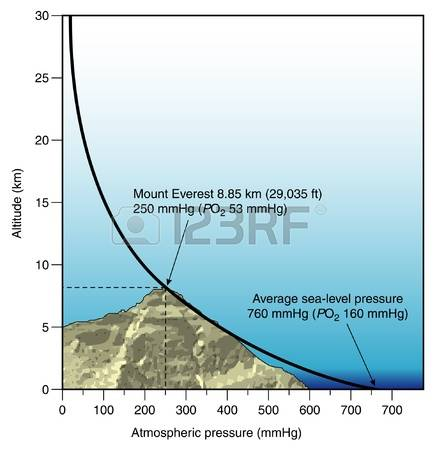
\includegraphics[width=8cm]{Presion}
\caption{\label{presion} Gráfica de altitud contra presión}
\end{figure}

\subsection{Temperatura y velocidad del sonido}
La división de la atmósfera es debido a la temperatura que experimenta.
Desde el nivel del mar hasta los 11 km de altitud la temperatura deciende
gradualmente, tras los 11 km se mantiene prácticamente constante durante
una gran distancia vertical en el resto de la troposfera. Posteriormente,
cerca de los 20 km, vuelve a incrementar debido a la captura de rayos UV
por la capa de ozono.
\\[3mm] En un gas ideal, la velocidad del sonido depende únicamente de
la temperatura y no de la presión o densidad, siendo así como lo hace
el sonido en nuestra atmósfera.

\subsection{Densidad y masa}
La densidad del aire a nivel del mar es alrededor $1.2 kg/m^{3}$.
En realidad la densidad no es medida sino calculada en base de la
temperatura, presión y humedad aplicando la ecuación de estado del
aire. Esta densidad disminuye mientras la altitud incrementa. Dichas
variaciones se modelan usando fórmulas barométricas.
\\[3mm] En promedio, la totalidad de masa presente en toda la
atmósfera es de $5x10^{15}$ toneladas. Según el Centro Nacional
Americano para la Investigación Atmosférica, la cantidad tiene
cierto rango debido al agua de $1.5x10^{15}$ kg, dependiendo de
la presión en el área.

\section{Propiedades ópticas}
La radiación solar es la energía que recibe la Tierra del Sol. El
planeta emite cierta radiación de vuelta pero nos es imperceptible.
Parte de esta radiación es absorbida y otra reflejada por la atmósfera.

\subsection{Disperción}
Cuando la luz pasa a través de la atmósfera, los fotones se dispersan
en ella. Si la luz no interacciona con la atmósfera entonces podemos
llamarle una radiación directa; en cambio, cuando los rayos de luz
han sido dispersados por la atmósfera se le llama radiación indirecta.
Es por ello que el cielo luce azul pues se debe a las ondas generados
por esta interacción y la tonalidad roja es aquella que presenta menos
dispersión.

\subsection{Absorción}
Las distintas moléculas absorben distintas longitudes de onda
de radiación (i.e. $O_2$ y $O_3$, longitudes menores a 300 nm
y $H_2 O$, mayores a 700 nm) . En el momento que un fotón es
absorbido, la molécula responsable incrementa su energía,
calentando así la atmósfera aunque también se enfría al emitir
radiación.
\\[3mm] El espectro que logra traspasar se encuentra entre los
400-700 nm y continua alrededor de los 1100 nm.

\subsection{Emisión}
La emisión es lo opuesto a la absorción, representa la emisión
de radiación. Esta tendencia de emisión depende de la emisión
de "cuerpo negro", es por ello que los cuerpos más calientes
emiten más radiación, con longitudes de onda muy cortas; mientras
que los más helados, emiten menos y en con una longitud muy grande.

\subsection{Índice de refracción}
El aire presenta un índice de refracción muy cercano pero superior
a 1. Esto puede ocasionar que se doblen los rayos de luz y hacer
ver objetos en el horizonte antes de que estén en la verdadera
posición.
\\ La temperatura es un factor que altera el índice de refracción,
haciendo que sean más notorios sus efectos cuando el gradiente de
temperatura es grande.
\\[3mm] La figura 3 es una puesta de sol, la cual resulta ser un gran
ejemplo del índice de refracción que presentan la radiación solar al
entrar en contacto con nuestra atmósfera.

\begin{figure}
\centering
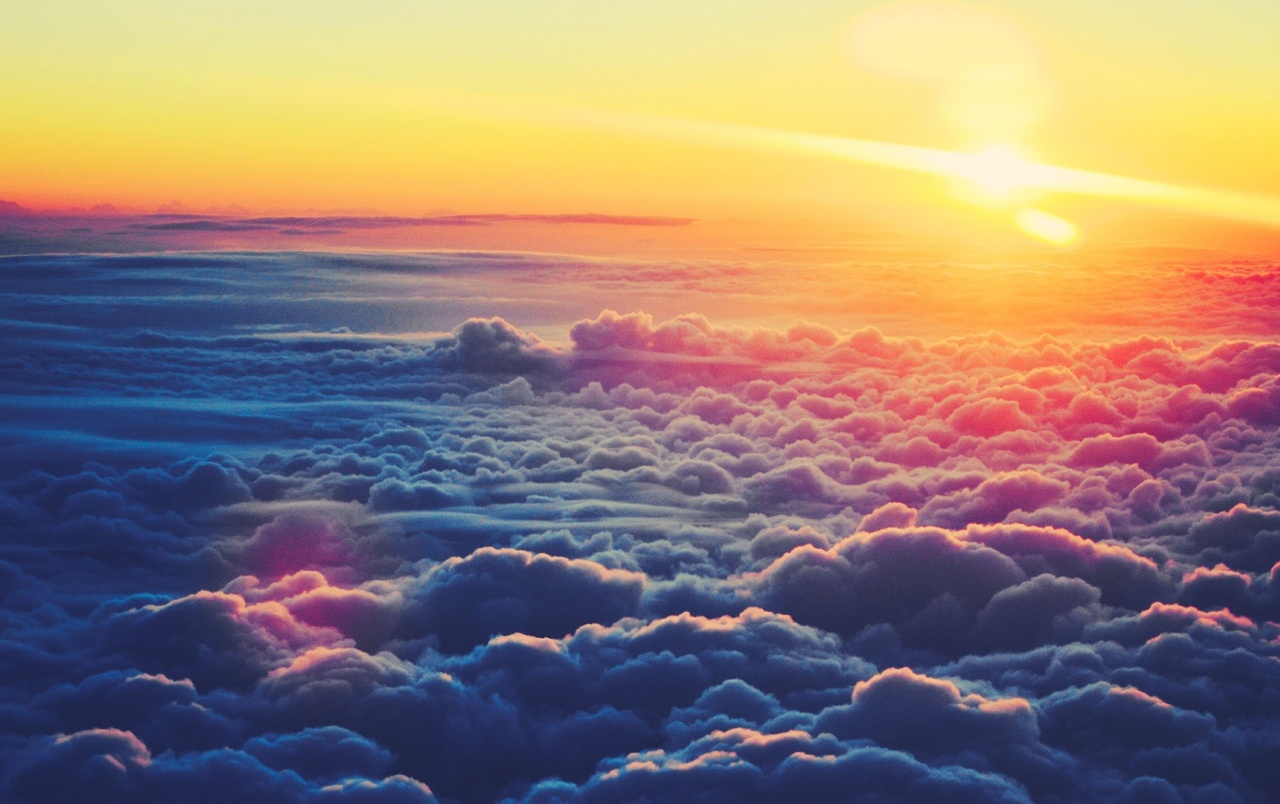
\includegraphics[width=7cm]{Puesta}
\caption{\label{puesta}Los colores generados dependen del índice de refracción.}
\end{figure}

\section{Circulación}
Circulación atmosférica es el movimiento a gran escala del aire a
través de la troposfera, y los medios por los cuales el calor se
distribuye alrededor de la Tierra. Este gran movimiento varía año
con año pero la estructura básica se mantiene prácticamente constante
ya que está determinado por la rotación del planeta y la diferencia
de radiación entre el ecuador y los polos.

\setlength\parindent{24pt}

\section{Apéndice}
\begin{itemize}
\item
¿Qué fue lo que más te llamó la atención de esta actividad?
\\[3mm] Lo más interesante de la actividad me pareció el hecho
de comenzar a aprender el cómo utilizar \LaTeX{} pues hace tiempo ya he
escuchado que es usado frecuentemente en el área de la ciencia.

\item
¿Qué fue lo que se te hizo menos interesante?
\\[3mm] Lo menos interesante me parece ser la lectura que se debe
realizar para llevar a cabo la actividad.

\item
¿Qué cambios harías para mejorar esta actividad?
\\[3mm] Sería buena idea que fuese un tema libre el cual expondremos en el
reporte y una guía más específica para cada sección del documento.
\\[3mm] También sería una buena idea recibir un par de clases explicando
previamente el tipo de funciones a utilizar en el archivo para ahorrar
tiempo al momento de trabajar en el reporte.

\item ¿Cuál es tu primera impresión de uso de \LaTeX?
\\[3mm] Me parece que es bastante complicado el crear documentos en esta
plataforma y de momento no me ha gustado dado esa "complejidad" que
encuentro en ello, preferiría utilizar un editor de textos, sin embargo no
niego que la apariencia del documento es muy interesante.

\item ¿El tiempo sugerido para esta actividad fue suficiente?
\\[3mm] Me parece que sido suficiente tiempo para trabajar en la actividad
pero de igual forma, si hubieramos tenido algo más de información puede
que hayamos tenido que usar menos.

\item ¿Encontraste algún documento o recurso en línea útil que quisieras compartir con los demás?
\\[3mm] No considero que hayan sido muy completa la información o que tuviera una buena estructura.
\end{itemize}

\section{Bibliografía}
\begin{itemize}
\item[$\circ$]
Atmosphere of Earth. Consultado el 29 de enero, 2018.
\\ https://en.wikipedia.org/wiki/Atmosphere\_of\_Earth
\\
\item[$\circ$]
Figura 1: Capas de la atmósfera.
\\ https://programacion167.files.wordpress.com/2016/08/2-atmosfera.png?w=700
\\
\item[$\circ$]
Figura 2: Presión atmosférica.
\\ https://us.123rf.com/450wm/hfsimaging/hfsimaging1201/hfsimaging120100022
\\/12092767-atmospheric-pressure-graph.jpg?ver=6
\\
\item[$\circ$]
Figura 3: Puesta de sol.
\\ https://wallpaperstock.net/wallpapers/thumbs1/35833hd.jpg

\end{itemize}

\end{document}
